% Options for packages loaded elsewhere
\PassOptionsToPackage{unicode}{hyperref}
\PassOptionsToPackage{hyphens}{url}
%
\documentclass[
]{article}
\usepackage{amsmath,amssymb}
\usepackage{lmodern}
\usepackage{ifxetex,ifluatex}
\ifnum 0\ifxetex 1\fi\ifluatex 1\fi=0 % if pdftex
  \usepackage[T1]{fontenc}
  \usepackage[utf8]{inputenc}
  \usepackage{textcomp} % provide euro and other symbols
\else % if luatex or xetex
  \usepackage{unicode-math}
  \defaultfontfeatures{Scale=MatchLowercase}
  \defaultfontfeatures[\rmfamily]{Ligatures=TeX,Scale=1}
\fi
% Use upquote if available, for straight quotes in verbatim environments
\IfFileExists{upquote.sty}{\usepackage{upquote}}{}
\IfFileExists{microtype.sty}{% use microtype if available
  \usepackage[]{microtype}
  \UseMicrotypeSet[protrusion]{basicmath} % disable protrusion for tt fonts
}{}
\makeatletter
\@ifundefined{KOMAClassName}{% if non-KOMA class
  \IfFileExists{parskip.sty}{%
    \usepackage{parskip}
  }{% else
    \setlength{\parindent}{0pt}
    \setlength{\parskip}{6pt plus 2pt minus 1pt}}
}{% if KOMA class
  \KOMAoptions{parskip=half}}
\makeatother
\usepackage{xcolor}
\IfFileExists{xurl.sty}{\usepackage{xurl}}{} % add URL line breaks if available
\IfFileExists{bookmark.sty}{\usepackage{bookmark}}{\usepackage{hyperref}}
\hypersetup{
  pdftitle={Assignment\_3},
  hidelinks,
  pdfcreator={LaTeX via pandoc}}
\urlstyle{same} % disable monospaced font for URLs
\usepackage[margin=1in]{geometry}
\usepackage{color}
\usepackage{fancyvrb}
\newcommand{\VerbBar}{|}
\newcommand{\VERB}{\Verb[commandchars=\\\{\}]}
\DefineVerbatimEnvironment{Highlighting}{Verbatim}{commandchars=\\\{\}}
% Add ',fontsize=\small' for more characters per line
\usepackage{framed}
\definecolor{shadecolor}{RGB}{248,248,248}
\newenvironment{Shaded}{\begin{snugshade}}{\end{snugshade}}
\newcommand{\AlertTok}[1]{\textcolor[rgb]{0.94,0.16,0.16}{#1}}
\newcommand{\AnnotationTok}[1]{\textcolor[rgb]{0.56,0.35,0.01}{\textbf{\textit{#1}}}}
\newcommand{\AttributeTok}[1]{\textcolor[rgb]{0.77,0.63,0.00}{#1}}
\newcommand{\BaseNTok}[1]{\textcolor[rgb]{0.00,0.00,0.81}{#1}}
\newcommand{\BuiltInTok}[1]{#1}
\newcommand{\CharTok}[1]{\textcolor[rgb]{0.31,0.60,0.02}{#1}}
\newcommand{\CommentTok}[1]{\textcolor[rgb]{0.56,0.35,0.01}{\textit{#1}}}
\newcommand{\CommentVarTok}[1]{\textcolor[rgb]{0.56,0.35,0.01}{\textbf{\textit{#1}}}}
\newcommand{\ConstantTok}[1]{\textcolor[rgb]{0.00,0.00,0.00}{#1}}
\newcommand{\ControlFlowTok}[1]{\textcolor[rgb]{0.13,0.29,0.53}{\textbf{#1}}}
\newcommand{\DataTypeTok}[1]{\textcolor[rgb]{0.13,0.29,0.53}{#1}}
\newcommand{\DecValTok}[1]{\textcolor[rgb]{0.00,0.00,0.81}{#1}}
\newcommand{\DocumentationTok}[1]{\textcolor[rgb]{0.56,0.35,0.01}{\textbf{\textit{#1}}}}
\newcommand{\ErrorTok}[1]{\textcolor[rgb]{0.64,0.00,0.00}{\textbf{#1}}}
\newcommand{\ExtensionTok}[1]{#1}
\newcommand{\FloatTok}[1]{\textcolor[rgb]{0.00,0.00,0.81}{#1}}
\newcommand{\FunctionTok}[1]{\textcolor[rgb]{0.00,0.00,0.00}{#1}}
\newcommand{\ImportTok}[1]{#1}
\newcommand{\InformationTok}[1]{\textcolor[rgb]{0.56,0.35,0.01}{\textbf{\textit{#1}}}}
\newcommand{\KeywordTok}[1]{\textcolor[rgb]{0.13,0.29,0.53}{\textbf{#1}}}
\newcommand{\NormalTok}[1]{#1}
\newcommand{\OperatorTok}[1]{\textcolor[rgb]{0.81,0.36,0.00}{\textbf{#1}}}
\newcommand{\OtherTok}[1]{\textcolor[rgb]{0.56,0.35,0.01}{#1}}
\newcommand{\PreprocessorTok}[1]{\textcolor[rgb]{0.56,0.35,0.01}{\textit{#1}}}
\newcommand{\RegionMarkerTok}[1]{#1}
\newcommand{\SpecialCharTok}[1]{\textcolor[rgb]{0.00,0.00,0.00}{#1}}
\newcommand{\SpecialStringTok}[1]{\textcolor[rgb]{0.31,0.60,0.02}{#1}}
\newcommand{\StringTok}[1]{\textcolor[rgb]{0.31,0.60,0.02}{#1}}
\newcommand{\VariableTok}[1]{\textcolor[rgb]{0.00,0.00,0.00}{#1}}
\newcommand{\VerbatimStringTok}[1]{\textcolor[rgb]{0.31,0.60,0.02}{#1}}
\newcommand{\WarningTok}[1]{\textcolor[rgb]{0.56,0.35,0.01}{\textbf{\textit{#1}}}}
\usepackage{graphicx}
\makeatletter
\def\maxwidth{\ifdim\Gin@nat@width>\linewidth\linewidth\else\Gin@nat@width\fi}
\def\maxheight{\ifdim\Gin@nat@height>\textheight\textheight\else\Gin@nat@height\fi}
\makeatother
% Scale images if necessary, so that they will not overflow the page
% margins by default, and it is still possible to overwrite the defaults
% using explicit options in \includegraphics[width, height, ...]{}
\setkeys{Gin}{width=\maxwidth,height=\maxheight,keepaspectratio}
% Set default figure placement to htbp
\makeatletter
\def\fps@figure{htbp}
\makeatother
\setlength{\emergencystretch}{3em} % prevent overfull lines
\providecommand{\tightlist}{%
  \setlength{\itemsep}{0pt}\setlength{\parskip}{0pt}}
\setcounter{secnumdepth}{-\maxdimen} % remove section numbering
\ifluatex
  \usepackage{selnolig}  % disable illegal ligatures
\fi

\title{Assignment\_3}
\author{}
\date{\vspace{-2.5em}}

\begin{document}
\maketitle

\hypertarget{r-markdown}{%
\subsection{R Markdown}\label{r-markdown}}

This is an R Markdown document. Markdown is a simple formatting syntax
for authoring HTML, PDF, and MS Word documents. For more details on
using R Markdown see \url{http://rmarkdown.rstudio.com}.

When you click the \textbf{Knit} button a document will be generated
that includes both content as well as the output of any embedded R code
chunks within the document. You can embed an R code chunk like this:

\begin{Shaded}
\begin{Highlighting}[]
\FunctionTok{summary}\NormalTok{(cars)}
\end{Highlighting}
\end{Shaded}

\begin{verbatim}
##      speed           dist       
##  Min.   : 4.0   Min.   :  2.00  
##  1st Qu.:12.0   1st Qu.: 26.00  
##  Median :15.0   Median : 36.00  
##  Mean   :15.4   Mean   : 42.98  
##  3rd Qu.:19.0   3rd Qu.: 56.00  
##  Max.   :25.0   Max.   :120.00
\end{verbatim}

\hypertarget{including-plots}{%
\subsection{Including Plots}\label{including-plots}}

You can also embed plots, for example:

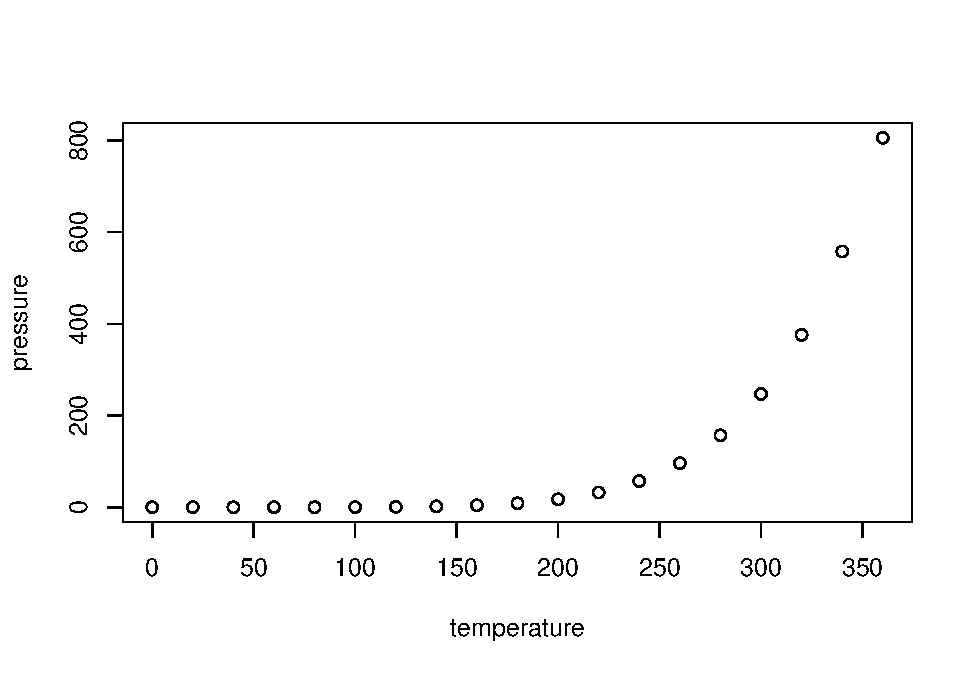
\includegraphics{Assignment_3_files/figure-latex/pressure-1.pdf}

Note that the \texttt{echo\ =\ FALSE} parameter was added to the code
chunk to prevent printing of the R code that generated the plot.

library(readr) library(dplyr) library(fastDummies) library(ggplot2)
library(caret) library(class)

install.packages(``lattice'')

UniversalBank \textless- read\_csv(``UniversalBank.csv'')
View(UniversalBank)

head(UniversalBank) summary(UniversalBank) glimpse(UniversalBank)

UniversalBank\(Education <- as.factor(UniversalBank\)Education)
UniversalBank2 \textless- UniversalBank UniversalBank2 \textless-
dummy\_cols(UniversalBank2 \%\textgreater\%
select(-c(ID,\texttt{ZIP\ Code},\texttt{Personal\ Loan})))
glimpse(UniversalBank2)

UniversalBank2 \textless- UniversalBank2 \%\textgreater\%
mutate(\texttt{Personal\ Loan}=UniversalBank\$\texttt{Personal\ Loan})
\%\textgreater\% select(-c(Education)) glimpse(UniversalBank2)
ggplot(UniversalBank, aes(x=\texttt{Personal\ Loan})) +
geom\_bar(fill=``blue'') + labs(title=``Bar Plot for Personal Loan'')

ggplot(UniversalBank, aes(x=Mortgage)) + geom\_histogram()
ggplot(UniversalBank, aes(x=\texttt{Personal\ Loan}, y=Income)) +
geom\_boxplot()

\hypertarget{data-partition-60-training-40-testing}{%
\section{Data partition 60\% training 40\%
testing}\label{data-partition-60-training-40-testing}}

set.seed(123) index \textless-
createDataPartition(UniversalBank2\$\texttt{Personal\ Loan}, p=0.6,
list=FALSE)

UniversalBank2\_train\_df \textless- UniversalBank2{[}index,{]}
UniversalBank2\_test\_df \textless- UniversalBank2{[}-index,{]}

glimpse(UniversalBank2\_train\_df) glimpse(UniversalBank2\_test\_df)

scale\_fun \textless- preProcess(UniversalBank2\_train\_df{[}-14{]},
method=c(``center'',``scale'')) (UniversalBank2\_test\_norm \textless-
predict(scale\_fun, UniversalBank2\_train\_df{[},-14{]}))
(UniversalBank2\_train\_norm \textless- predict(scale\_fun,
UniversalBank2\_test\_df{[},-14{]}))

\hypertarget{knn-model-start-here-input-variable-x-and-y-cl}{%
\section{knn model start here input variable x and y cl
=}\label{knn-model-start-here-input-variable-x-and-y-cl}}

install.packages(``pivottabler'') library(pivottabler)

summary(UniversalBank2\_train\_df)

? melt

\hypertarget{fast-melt-a-data.table}{%
\subsection{fast melt a data.table}\label{fast-melt-a-data.table}}

\hypertarget{s3-method-for-class-data.table}{%
\subsection{S3 method for class
`data.table'}\label{s3-method-for-class-data.table}}

\hypertarget{meltdata-id.vars-measure.vars}{%
\subsection{melt(data, id.vars,
measure.vars,}\label{meltdata-id.vars-measure.vars}}

\begin{verbatim}
variable.name = "variable", value.name = "value",
..., na.rm = FALSE, variable.factor = TRUE,
value.factor = FALSE,
verbose = getOption("datatable.verbose"))
\end{verbatim}

install.packages(``tidyverse'') library(tidyverse)

library(readxl) install.packages(``here'') library(here)
install.packages(``skimr'') library(skimr)

install.packages(``reshape2'') library(reshape2)

\hypertarget{testing-an-example-that-i-found-to-see-how-this-works}{%
\subsection{testing an example that I found to see how this
works}\label{testing-an-example-that-i-found-to-see-how-this-works}}

country\textless-data.frame(c(``A'',``B'',``C''),c(100,200,120),c(2000,7000,15000))
colnames(country)\textless-
c(``countries'',``population\_in\_million'',``gdp\_percapita'')

\hypertarget{melt-function-in-r}{%
\subparagraph{melt() function in R}\label{melt-function-in-r}}

country\_w\_to\_L = melt(country, id.vars=c(``countries''))

country\_w\_to\_L

long to wide using cast function of reshape2() package in R

country\_L\_to\_W = dcast(country\_w\_to\_L,
countries\textasciitilde variable,sum)

country\_L\_to\_W

\hypertarget{trying-this-with-universalbank-files-in-my-environment}{%
\subsubsection{Trying this with universalbank files in my
environment}\label{trying-this-with-universalbank-files-in-my-environment}}

UniversalBank2\_train\_norm\_w\_to\_L =
melt(UniversalBank2\_train\_norm, id.vars=c(``Online'',``CreditCard''))

UniversalBank2\_train\_df\_w\_to\_L = melt(UniversalBank2\_train\_df,
id.vars=c(``Online'',``CreditCard'',``Personal Loan''))

UniversalBank2\_train\_df\_w\_to\_L
summary(UniversalBank2\_train\_df\_w\_to\_L)

\hypertarget{there-is-something-wrong-with-this}{%
\subsection{There is something wrong with
this}\label{there-is-something-wrong-with-this}}

UniversalBank2\_train\_df\_L\_to\_W =
dcast(UniversalBank2\_train\_df\_w\_to\_L,
UniversalBank2\_train\_df\_w\_to\_L\textasciitilde variable,count)

UniversalBank2\_train\_df\_L\_to\_W

\hypertarget{im-getting-errors}{%
\subsubsection{I'm getting errors}\label{im-getting-errors}}

\hypertarget{error-cant-subset-columns-that-dont-exist.}{%
\section{Error: Can't subset columns that don't
exist.}\label{error-cant-subset-columns-that-dont-exist.}}

\hypertarget{x-locations-4558-5568-5699-3185-3461-etc.-dont-exist.}{%
\section{x Locations 4558, 5568, 5699, 3185, 3461, etc. don't
exist.}\label{x-locations-4558-5568-5699-3185-3461-etc.-dont-exist.}}

\hypertarget{i-there-are-only-14-columns.}{%
\section{i There are only 14
columns.}\label{i-there-are-only-14-columns.}}

\hypertarget{run-rlanglast_error-to-see-where-the-error-occurred.}{%
\section{\texorpdfstring{Run \texttt{rlang::last\_error()} to see where
the error
occurred.}{Run rlang::last\_error() to see where the error occurred.}}\label{run-rlanglast_error-to-see-where-the-error-occurred.}}

\hypertarget{in-addition-warning-message}{%
\section{In addition: Warning
message:}\label{in-addition-warning-message}}

\hypertarget{in-xtfrm.data.framex-cannot-xtfrm-data-frames}{%
\section{In xtfrm.data.frame(x) : cannot xtfrm data
frames}\label{in-xtfrm.data.framex-cannot-xtfrm-data-frames}}

\hypertarget{universalbank2_train_df_l_to_w}{%
\section{\textgreater{}
UniversalBank2\_train\_df\_L\_to\_W}\label{universalbank2_train_df_l_to_w}}

\hypertarget{error-object-universalbank2_train_df_l_to_w-not-found}{%
\section{Error: object `UniversalBank2\_train\_df\_L\_to\_W' not
found}\label{error-object-universalbank2_train_df_l_to_w-not-found}}

\hypertarget{universalbank2_train_df_l_to_w-dcastuniversalbank2_train_df_w_to_l-universalbank2_train_df_w_to_lvariablecount}{%
\section{\textgreater{} UniversalBank2\_train\_df\_L\_to\_W =
dcast(UniversalBank2\_train\_df\_w\_to\_L, \#
UniversalBank2\_train\_df\_w\_to\_L\textasciitilde variable,count)}\label{universalbank2_train_df_l_to_w-dcastuniversalbank2_train_df_w_to_l-universalbank2_train_df_w_to_lvariablecount}}

\hypertarget{error-in-.data.framex-orderx-na.last-na.last-decreasing-decreasing}{%
\section{\texorpdfstring{Error in \texttt{{[}.data.frame}(x, order(x,
na.last = na.last, decreasing = decreasing))
:}{Error in {[}.data.frame(x, order(x, na.last = na.last, decreasing = decreasing)) :}}\label{error-in-.data.framex-orderx-na.last-na.last-decreasing-decreasing}}

\hypertarget{undefined-columns-selected}{%
\section{undefined columns selected}\label{undefined-columns-selected}}

\hypertarget{in-addition-warning-message-1}{%
\section{In addition: Warning
message:}\label{in-addition-warning-message-1}}

\hypertarget{in-xtfrm.data.framex-cannot-xtfrm-data-frames-1}{%
\section{In xtfrm.data.frame(x) : cannot xtfrm data
frames}\label{in-xtfrm.data.framex-cannot-xtfrm-data-frames-1}}

\hypertarget{there-is-something-wrong-with-this---trying-to-figure-it-out}{%
\subsection{There is something wrong with this - trying to figure it
out}\label{there-is-something-wrong-with-this---trying-to-figure-it-out}}

UniversalBank2\_train\_df\_L\_to\_W =
dcast(UniversalBank2\_train\_df\_w\_to\_L,
UniversalBank2\_train\_df\_w\_to\_L\textasciitilde variable,count)

UniversalBank2\_train\_df\_L\_to\_W

UniversalBank2\_train\_df\_L\_to\_W =
dcast(UniversalBank2\_train\_df\_w\_to\_L,
UniversalBank2\_train\_df\textasciitilde variable,sum)

rlang::last\_error() rlang::last\_trace()

\hypertarget{still-cant-figure-this-out}{%
\section{still can't figure this out}\label{still-cant-figure-this-out}}

UniversalBank2\_train\_df\_L\_to\_W =
dcast(UniversalBank2\_train\_df\_w\_to\_L,
id.vars=c(``Online'',``CreditCard'',``Personal Loan''))

UniversalBank2\_train\_df\_w\_to\_L
summary(UniversalBank2\_train\_df\_w\_to\_L)

UniversalBank2\_train\_df\_L\_to\_W =
dcast(UniversalBank2\_train\_df\_w\_to\_L,
UniversalBank2\_train\_norm\textasciitilde variable,count)

pivot(UniversalBank2\_train\_df\_w\_to\_L)
dcast(UniversalBank2\_train\_df\_w\_to\_L)
table(UniversalBank2\_train\_df\_w\_to\_L)
table(UniversalBank2\_train\_df\_w\_to\_L\(CreditCard) table(UniversalBank2_train_df_w_to_L\)Online)

head(UniversalBank2\_train\_df\_w\_to\_L)

library(dplyr)

UniversalBank2\_train\_df\_L\_to\_W =
dcast(UniversalBank2\_train\_df\_w\_to\_L,CreditCard\textasciitilde variable,
sum)

UniversalBank2\_train\_df\_L\_to\_W

\hypertarget{something-started-working-but-count-is-giving-me-grief---i-can-do-pivots-in-excel-but-r-is-just-a-pain}{%
\paragraph{something started working but count is giving me grief - I
can do pivots in excel but R is just a
pain}\label{something-started-working-but-count-is-giving-me-grief---i-can-do-pivots-in-excel-but-r-is-just-a-pain}}

\hypertarget{universalbank2_train_df_l_to_w-dcastuniversalbank2_train_df_w_to_lonlinevariable-count}{%
\section{\textgreater{} UniversalBank2\_train\_df\_L\_to\_W =
dcast(UniversalBank2\_train\_df\_w\_to\_L,Online\textasciitilde variable,
count)}\label{universalbank2_train_df_l_to_w-dcastuniversalbank2_train_df_w_to_lonlinevariable-count}}

\hypertarget{error-in-usemethodcount}{%
\section{Error in UseMethod(``count'')
:}\label{error-in-usemethodcount}}

\hypertarget{no-applicable-method-for-count-applied-to-an-object-of-class-cdouble-numeric}{%
\section{no applicable method for `count' applied to an object of class
``c(`double',
`numeric')''}\label{no-applicable-method-for-count-applied-to-an-object-of-class-cdouble-numeric}}

\hypertarget{universalbank2_train_df_l_to_w-1}{%
\section{\textgreater{}
UniversalBank2\_train\_df\_L\_to\_W}\label{universalbank2_train_df_l_to_w-1}}

\hypertarget{online-age-experience-income-family-ccavg-mortgage-securities-account-cd-account}{%
\section{Online Age Experience Income Family CCAvg Mortgage Securities
Account CD
Account}\label{online-age-experience-income-family-ccavg-mortgage-securities-account-cd-account}}

1 0 54339 24049 86744 2898 2312.20 64774 125 12 2 1 81947 36568 133443
4299 3459.62 101085 184 165 \# Education\_1 Education\_2 Education\_3 1
526 321 354 2 746 534 519 \#\textgreater{}
UniversalBank2\_train\_df\_L\_to\_W =
dcast(UniversalBank2\_train\_df\_w\_to\_L,Online\textasciitilde variable,
sum) \#\textgreater{} UniversalBank2\_train\_df\_L\_to\_W Online Age
Experience Income Family CCAvg Mortgage Securities Account CD Account 1
0 54339 24049 86744 2898 2312.20 64774 125 12 2 1 81947 36568 133443
4299 3459.62 101085 184 165 Education\_1 Education\_2 Education\_3 1 526
321 354 2 746 534 519 \# \textgreater{}
UniversalBank2\_train\_df\_L\_to\_W =
dcast(UniversalBank2\_train\_df\_w\_to\_L,Personal
Loan\textasciitilde variable, sum) \# Error: unexpected symbol in
``UniversalBank2\_train\_df\_L\_to\_W =
dcast(UniversalBank2\_train\_df\_w\_to\_L,Personal Loan'' \#
\textgreater{} UniversalBank2\_train\_df\_L\_to\_W =
dcast(UniversalBank2\_train\_df\_w\_to\_L,CreditCard\textasciitilde variable,
sum) \# \textgreater{} UniversalBank2\_train\_df\_L\_to\_W CreditCard
Age Experience Income Family CCAvg Mortgage Securities Account 1 0 95969
42547 153620 5098 4049.85 116296 231 2 1 40317 18070 66567 2099 1721.97
49563 78 CD Account Education\_1 Education\_2 Education\_3 1 33 891 607
619 2 144 381 248 254

\hypertarget{compute-the-following-quantities-pa-b-means-the-probability-ofa-given-b-i.-pcc-1-loan-1-the-proportion-of-credit-card-holders-among-the-loan-acceptors-ii.-ponline-1-loan-1-iii.-ploan-1-the-proportion-of-loan-acceptors-iv.-pcc-1-loan-0-v.-ponline-1-loan-0-vi.-ploan-0}{%
\subsubsection{Compute the following quantities {[}P(A \textbar{} B)
means ``the probability ofA given B''{]}: i. P(CC = 1 \textbar{} Loan =
1) (the proportion of credit card holders among the loan acceptors) ii.
P(Online = 1 \textbar{} Loan = 1) iii. P(Loan = 1) (the proportion of
loan acceptors) iv. P(CC = 1 \textbar{} Loan = 0) v. P(Online = 1
\textbar{} Loan = 0) vi. P(Loan =
0)}\label{compute-the-following-quantities-pa-b-means-the-probability-ofa-given-b-i.-pcc-1-loan-1-the-proportion-of-credit-card-holders-among-the-loan-acceptors-ii.-ponline-1-loan-1-iii.-ploan-1-the-proportion-of-loan-acceptors-iv.-pcc-1-loan-0-v.-ponline-1-loan-0-vi.-ploan-0}}

\hypertarget{output-file-assignment_3.knit.md}{%
\section{output file:
Assignment\_3.knit.md}\label{output-file-assignment_3.knit.md}}

\hypertarget{cprogram-filesrstudiobinpandocpandoc-rts--k512m--rts-assignment_3.knit.md-to-latex-from-markdownautolink_bare_uristex_math_single_backslash-output-assignment_3.tex-lua-filter-c-library4.1.lua-lua-filter-c-library4.1-div.lua-self-contained-highlight-style-tango-pdf-engine-pdflatex-variable-graphics-variable-geometrymargin1in}{%
\section{\texorpdfstring{``C:/Program Files/RStudio/bin/pandoc/pandoc''
+RTS -K512m -RTS Assignment\_3.knit.md --to latex --from
markdown+autolink\_bare\_uris+tex\_math\_single\_backslash --output
Assignment\_3.tex --lua-filter
``C:\Users\xlamo\Documents\R\win-library\textbackslash4.1\rmarkdown\rmarkdown\lua\pagebreak.lua''
--lua-filter
``C:\Users\xlamo\Documents\R\win-library\textbackslash4.1\rmarkdown\rmarkdown\lua\latex-div.lua''
--self-contained --highlight-style tango --pdf-engine pdflatex
--variable graphics --variable
``geometry:margin=1in''}{``C:/Program Files/RStudio/bin/pandoc/pandoc'' +RTS -K512m -RTS Assignment\_3.knit.md --to latex --from markdown+autolink\_bare\_uris+tex\_math\_single\_backslash --output Assignment\_3.tex --lua-filter ``C:-library\textbackslash4.1.lua'' --lua-filter ``C:-library\textbackslash4.1-div.lua'' --self-contained --highlight-style tango --pdf-engine pdflatex --variable graphics --variable ``geometry:margin=1in''}}\label{cprogram-filesrstudiobinpandocpandoc-rts--k512m--rts-assignment_3.knit.md-to-latex-from-markdownautolink_bare_uristex_math_single_backslash-output-assignment_3.tex-lua-filter-c-library4.1.lua-lua-filter-c-library4.1-div.lua-self-contained-highlight-style-tango-pdf-engine-pdflatex-variable-graphics-variable-geometrymargin1in}}

\hypertarget{double-subscript.}{%
\section{! Double subscript.}\label{double-subscript.}}

\hypertarget{l.364-ditcard-tableuniversalbank2_train_df_w_}{%
\section{l.364 \ldots ditCard)
table(UniversalBank2\_train\_df\_w\_}\label{l.364-ditcard-tableuniversalbank2_train_df_w_}}

\begin{verbatim}
                                              to_L\)Online) 
\end{verbatim}

\hypertarget{error-latex-failed-to-compile-assignment_3.tex.-see-httpsyihui.orgtinytexrdebugging-for-debugging-tips.-see-assignment_3.log-for-more-info.}{%
\section{\texorpdfstring{Error: LaTeX failed to compile
Assignment\_3.tex. See \url{https://yihui.org/tinytex/r/\#debugging} for
debugging tips. See Assignment\_3.log for more
info.}{Error: LaTeX failed to compile Assignment\_3.tex. See https://yihui.org/tinytex/r/\#debugging for debugging tips. See Assignment\_3.log for more info.}}\label{error-latex-failed-to-compile-assignment_3.tex.-see-httpsyihui.orgtinytexrdebugging-for-debugging-tips.-see-assignment_3.log-for-more-info.}}

\hypertarget{execution-halted}{%
\section{Execution halted}\label{execution-halted}}

\hypertarget{this-was-the-same-problem-i-kept-having-with-assignment_2-everything-kept-failing-and-execution-halted---this-is-frustrating}{%
\subparagraph{This was the same problem I kept having with Assignment\_2
--- everything kept failing and Execution Halted - this is
frustrating}\label{this-was-the-same-problem-i-kept-having-with-assignment_2-everything-kept-failing-and-execution-halted---this-is-frustrating}}

\end{document}
